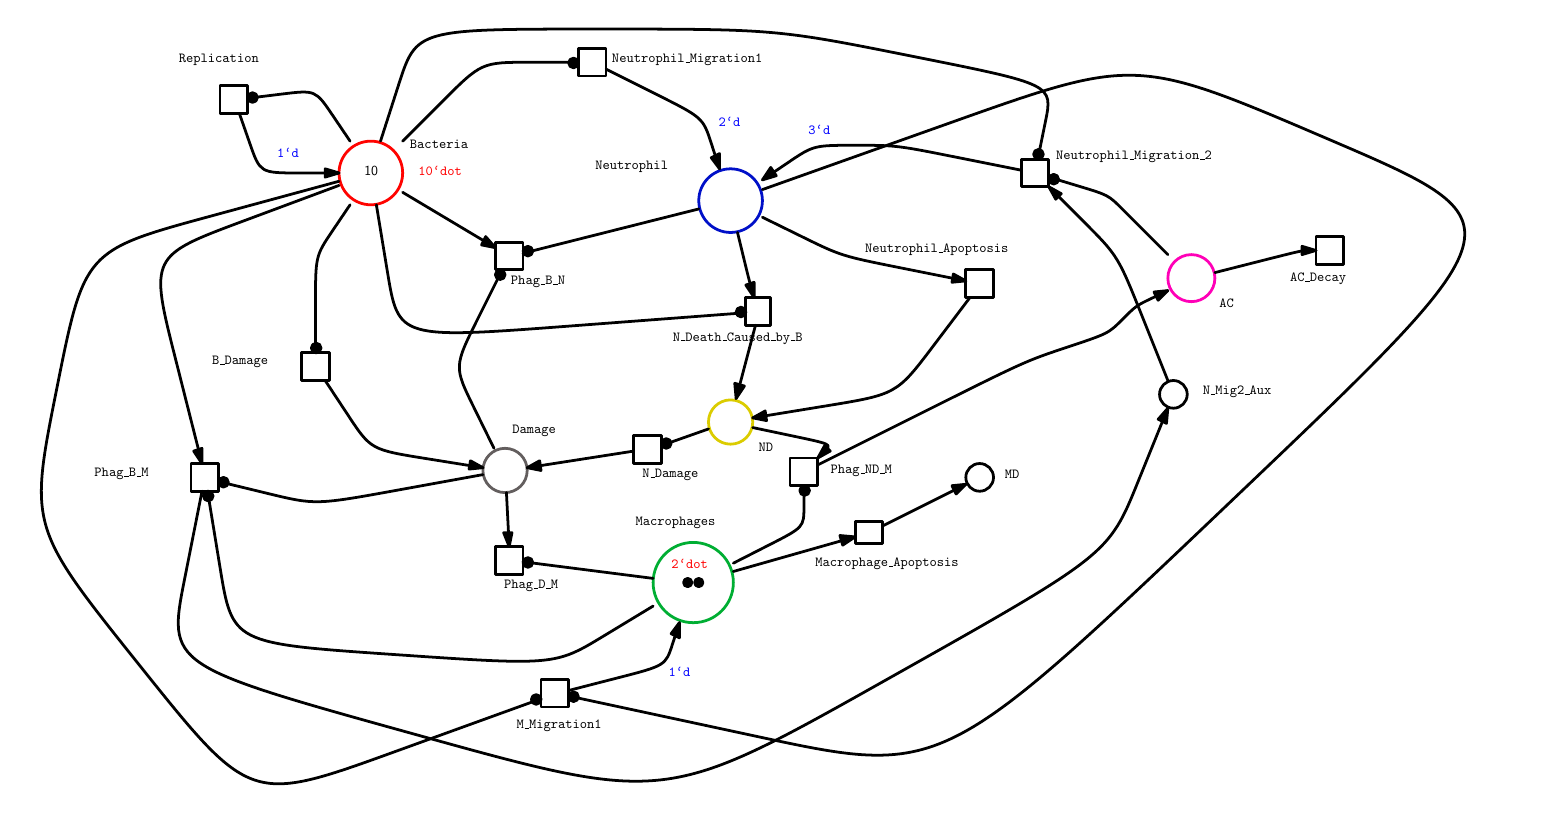
\begin{tikzpicture}[x=1pt,y=-1pt,scale=0.5,transform shape]

\definecolor{r255g3b0}{RGB}{255,3,0}
\definecolor{WHITE}{RGB}{255,255,255}
\draw[r255g3b0, solid, line join=round, line cap=round, line width=1, fill=WHITE]
	(287,124) ellipse[x radius=23, y radius=23];
\definecolor{BLACK}{RGB}{0,0,0}
\draw[BLACK]
	(279,122.5) node[rotate=0, font=\sffamily\normalsize, BLACK, right=-.25]
	{10};
\draw[BLACK]
	(312,103.5) node[rotate=0, font=\ttfamily\normalsize, BLACK, right=-.25]
	{Bacteria};
\definecolor{RED}{RGB}{255,0,0}
\draw[BLACK]
	(318,122.5) node[rotate=0, font=\ttfamily\normalsize, RED, right=-.25]
	{10`dot};
\definecolor{r0g16b200}{RGB}{0,16,200}
\draw[r0g16b200, solid, line join=round, line cap=round, line width=1, fill=WHITE]
	(547,144) ellipse[x radius=23, y radius=23];
\draw[BLACK]
	(446,119.5) node[rotate=0, font=\ttfamily\normalsize, BLACK, right=-.25]
	{Neutrophil};
\definecolor{r99g94b94}{RGB}{99,94,94}
\draw[r99g94b94, solid, line join=round, line cap=round, line width=1, fill=WHITE]
	(384,339) ellipse[x radius=16, y radius=16];
\draw[BLACK]
	(386,310.5) node[rotate=0, font=\ttfamily\normalsize, BLACK, right=-.25]
	{Damage};
\definecolor{r219g204b0}{RGB}{219,204,0}
\draw[r219g204b0, solid, line join=round, line cap=round, line width=1, fill=WHITE]
	(547,304) ellipse[x radius=16, y radius=16];
\draw[BLACK]
	(564,322.5) node[rotate=0, font=\ttfamily\normalsize, BLACK, right=-.25]
	{ND};
\definecolor{r0g174b51}{RGB}{0,174,51}
\draw[r0g174b51, solid, line join=round, line cap=round, line width=1, fill=WHITE]
	(520,420) ellipse[x radius=29, y radius=29];
\draw[BLACK, solid, line join=round, line cap=round, line width=1, fill=BLACK]
	(516,420) ellipse[x radius=3, y radius=3];
\draw[BLACK, solid, line join=round, line cap=round, line width=1, fill=BLACK]
	(524,420) ellipse[x radius=3, y radius=3];
\draw[BLACK]
	(475,376.5) node[rotate=0, font=\ttfamily\normalsize, BLACK, right=-.25]
	{Macrophages};
\draw[BLACK]
	(501,406.5) node[rotate=0, font=\ttfamily\normalsize, RED, right=-.25]
	{2`dot};
\draw[BLACK, solid, line join=round, line cap=round, line width=1, fill=WHITE]
	(867,284) ellipse[x radius=10, y radius=10];
\draw[BLACK]
	(885,282.5) node[rotate=0, font=\ttfamily\normalsize, BLACK, right=-.25]
	{N\_Mig2\_Aux};
\draw[BLACK, solid, line join=round, line cap=round, line width=1, fill=WHITE]
	(727,344) ellipse[x radius=10, y radius=10];
\draw[BLACK]
	(742,341.5) node[rotate=0, font=\ttfamily\normalsize, BLACK, right=-.25]
	{MD};
\definecolor{r255g0b183}{RGB}{255,0,183}
\draw[r255g0b183, solid, line join=round, line cap=round, line width=1, fill=WHITE]
	(880,200) ellipse[x radius=17, y radius=17];
\draw[BLACK]
	(897,218.5) node[rotate=0, font=\ttfamily\normalsize, BLACK, right=-.25]
	{AC};
\draw[BLACK, solid, line join=round, line cap=round, line width=1, fill=WHITE]
	(178,61) rectangle +(20,20);
\draw[BLACK]
	(145,42.5) node[rotate=0, font=\ttfamily\normalsize, BLACK, right=-.25]
	{Replication};
\draw[BLACK, solid, line join=round, line cap=round, line width=1, fill=WHITE]
	(377,174) rectangle +(20,20);
\draw[BLACK]
	(385,202.5) node[rotate=0, font=\ttfamily\normalsize, BLACK, right=-.25]
	{Phag\_B\_N};
\draw[BLACK, solid, line join=round, line cap=round, line width=1, fill=WHITE]
	(558,214) rectangle +(18,20);
\draw[BLACK]
	(502,243.5) node[rotate=0, font=\ttfamily\normalsize, BLACK, right=-.25]
	{N\_Death\_Caused\_by\_B};
\draw[BLACK, solid, line join=round, line cap=round, line width=1, fill=WHITE]
	(477,314) rectangle +(20,20);
\draw[BLACK]
	(480,342.5) node[rotate=0, font=\ttfamily\normalsize, BLACK, right=-.25]
	{N\_Damage};
\draw[BLACK, solid, line join=round, line cap=round, line width=1, fill=WHITE]
	(237,254) rectangle +(20,20);
\draw[BLACK]
	(169,260.5) node[rotate=0, font=\ttfamily\normalsize, BLACK, right=-.25]
	{B\_Damage};
\draw[BLACK, solid, line join=round, line cap=round, line width=1, fill=WHITE]
	(377,394) rectangle +(20,20);
\draw[BLACK]
	(380,422.5) node[rotate=0, font=\ttfamily\normalsize, BLACK, right=-.25]
	{Phag\_D\_M};
\draw[BLACK, solid, line join=round, line cap=round, line width=1, fill=WHITE]
	(157,334) rectangle +(20,20);
\draw[BLACK]
	(84,341.5) node[rotate=0, font=\ttfamily\normalsize, BLACK, right=-.25]
	{Phag\_B\_M};
\draw[BLACK, solid, line join=round, line cap=round, line width=1, fill=WHITE]
	(757,114) rectangle +(20,20);
\draw[BLACK]
	(779,112.5) node[rotate=0, font=\ttfamily\normalsize, BLACK, right=-.25]
	{Neutrophil\_Migration\_2};
\draw[BLACK, solid, line join=round, line cap=round, line width=1, fill=WHITE]
	(717,194) rectangle +(20,20);
\draw[BLACK]
	(641,179.5) node[rotate=0, font=\ttfamily\normalsize, BLACK, right=-.25]
	{Neutrophil\_Apoptosis};
\draw[BLACK, solid, line join=round, line cap=round, line width=1, fill=WHITE]
	(637,376) rectangle +(20,16);
\draw[BLACK]
	(605,406.5) node[rotate=0, font=\ttfamily\normalsize, BLACK, right=-.25]
	{Macrophage\_Apoptosis};
\draw[BLACK, solid, line join=round, line cap=round, line width=1, fill=WHITE]
	(437,34) rectangle +(20,20);
\draw[BLACK]
	(458,42.5) node[rotate=0, font=\ttfamily\normalsize, BLACK, right=-.25]
	{Neutrophil\_Migration1};
\draw[BLACK, solid, line join=round, line cap=round, line width=1, fill=WHITE]
	(410,490) rectangle +(20,20);
\draw[BLACK]
	(389,523.5) node[rotate=0, font=\ttfamily\normalsize, BLACK, right=-.25]
	{M\_Migration1};
\draw[BLACK, solid, line join=round, line cap=round, line width=1, fill=WHITE]
	(590,330) rectangle +(20,20);
\draw[BLACK]
	(616,339.5) node[rotate=0, font=\ttfamily\normalsize, BLACK, right=-.25]
	{Phag\_ND\_M};
\draw[BLACK, solid, line join=round, line cap=round, line width=1, fill=WHITE]
	(970,170) rectangle +(20,20);
\draw[BLACK]
	(948,200.5) node[rotate=0, font=\ttfamily\normalsize, BLACK, right=-.25]
	{AC\_Decay};
\draw[BLACK, solid, line join=round, line cap=round, line width=1]
	(192,81) -- (199.5,102.5) .. controls (207,124) .. (235.5,124) -- (264,124);
\draw[BLACK, solid, line join=round, line cap=round, line width=1, fill=BLACK]
	(264,124) -- (254,127) -- (254,121) -- (264,124) -- cycle;
\definecolor{BLUE}{RGB}{0,0,255}
\draw[BLACK]
	(216,109.5) node[rotate=0, font=\ttfamily\normalsize, BLUE, right=-.25]
	{1`d};
\draw[BLACK, solid, line join=round, line cap=round, line width=1]
	(310,138) -- (377,178);
\draw[BLACK, solid, line join=round, line cap=round, line width=1, fill=BLACK]
	(377,178) -- (367,176) -- (370,170) -- (377,178) -- cycle;
\draw[BLACK, solid, line join=round, line cap=round, line width=1]
	(552,167) -- (556,183.5) .. controls (560,200) .. (562,207) -- (564,214);
\draw[BLACK, solid, line join=round, line cap=round, line width=1, fill=BLACK]
	(564,214) -- (558,205) -- (564,203) -- (564,214) -- cycle;
\draw[BLACK, solid, line join=round, line cap=round, line width=1]
	(565,234) -- (551,287);
\draw[BLACK, solid, line join=round, line cap=round, line width=1, fill=BLACK]
	(551,287) -- (550,276) -- (557,278) -- (551,287) -- cycle;
\draw[BLACK, solid, line join=round, line cap=round, line width=1]
	(477,325) -- (400,337);
\draw[BLACK, solid, line join=round, line cap=round, line width=1, fill=BLACK]
	(400,337) -- (409,332) -- (410,339) -- (400,337) -- cycle;
\draw[BLACK, solid, line join=round, line cap=round, line width=1]
	(254,274) -- (270.5,299) .. controls (287,324) .. (327.5,330.5) -- (368,337);
\draw[BLACK, solid, line join=round, line cap=round, line width=1, fill=BLACK]
	(368,337) -- (358,338) -- (359,332) -- (368,337) -- cycle;
\draw[BLACK, solid, line join=round, line cap=round, line width=1]
	(385,355) -- (387,394);
\draw[BLACK, solid, line join=round, line cap=round, line width=1, fill=BLACK]
	(387,394) -- (383,384) -- (389,384) -- (387,394) -- cycle;
\draw[BLACK, solid, line join=round, line cap=round, line width=1]
	(264,133) -- (195.5,158.5) .. controls (127,184) .. (146,259) -- (165,334);
\draw[BLACK, solid, line join=round, line cap=round, line width=1, fill=BLACK]
	(165,334) -- (159,325) -- (165,323) -- (165,334) -- cycle;
\draw[BLACK, solid, line join=round, line cap=round, line width=1]
	(757,122) -- (712,113) .. controls (667,104) .. (637,104) .. controls (607,104) .. (588.5,116.5) -- (570,129);
\draw[BLACK, solid, line join=round, line cap=round, line width=1, fill=BLACK]
	(570,129) -- (576,120) -- (580,126) -- (570,129) -- cycle;
\draw[BLACK]
	(600,93.5) node[rotate=0, font=\ttfamily\normalsize, BLUE, right=-.25]
	{3`d};
\draw[BLACK, solid, line join=round, line cap=round, line width=1]
	(165,354) -- (152.5,417) .. controls (140,480) .. (320,530) .. controls (500,580) .. (660,490) .. controls (820,400) .. (841.5,347) -- (863,294);
\draw[BLACK, solid, line join=round, line cap=round, line width=1, fill=BLACK]
	(863,294) -- (862,305) -- (856,302) -- (863,294) -- cycle;
\draw[BLACK, solid, line join=round, line cap=round, line width=1]
	(863,274) -- (845,229) .. controls (827,184) .. (802,159) -- (777,134);
\draw[BLACK, solid, line join=round, line cap=round, line width=1, fill=BLACK]
	(777,134) -- (786,139) -- (782,143) -- (777,134) -- cycle;
\draw[BLACK, solid, line join=round, line cap=round, line width=1]
	(570,156) -- (598.5,170) .. controls (627,184) .. (672,193) -- (717,202);
\draw[BLACK, solid, line join=round, line cap=round, line width=1, fill=BLACK]
	(717,202) -- (707,203) -- (708,197) -- (717,202) -- cycle;
\draw[BLACK, solid, line join=round, line cap=round, line width=1]
	(720,214) -- (693.5,249) .. controls (667,284) .. (615,292.5) -- (563,301);
\draw[BLACK, solid, line join=round, line cap=round, line width=1, fill=BLACK]
	(563,301) -- (572,296) -- (573,303) -- (563,301) -- cycle;
\draw[BLACK, solid, line join=round, line cap=round, line width=1]
	(549,412) -- (637,387);
\draw[BLACK, solid, line join=round, line cap=round, line width=1, fill=BLACK]
	(637,387) -- (628,393) -- (626,386) -- (637,387) -- cycle;
\draw[BLACK, solid, line join=round, line cap=round, line width=1]
	(657,379) -- (717,349);
\draw[BLACK, solid, line join=round, line cap=round, line width=1, fill=BLACK]
	(717,349) -- (710,356) -- (707,350) -- (717,349) -- cycle;
\draw[BLACK, solid, line join=round, line cap=round, line width=1]
	(457,49) -- (492,66.5) .. controls (527,84) .. (533,102.5) -- (539,121);
\draw[BLACK, solid, line join=round, line cap=round, line width=1, fill=BLACK]
	(539,121) -- (533,113) -- (539,110) -- (539,121) -- cycle;
\draw[BLACK]
	(535,87.5) node[rotate=0, font=\ttfamily\normalsize, BLUE, right=-.25]
	{2`d};
\draw[BLACK, solid, line join=round, line cap=round, line width=1]
	(430,498) -- (465,489) .. controls (500,480) .. (505,464.5) -- (510,449);
\draw[BLACK, solid, line join=round, line cap=round, line width=1, fill=BLACK]
	(510,449) -- (510,460) -- (504,457) -- (510,449) -- cycle;
\draw[BLACK]
	(499,484.5) node[rotate=0, font=\ttfamily\normalsize, BLUE, right=-.25]
	{1`d};
\draw[BLACK, solid, line join=round, line cap=round, line width=1]
	(563,308) -- (591.5,314) .. controls (620,320) .. (615,325) -- (610,330);
\draw[BLACK, solid, line join=round, line cap=round, line width=1, fill=BLACK]
	(610,330) -- (615,321) -- (619,325) -- (610,330) -- cycle;
\draw[BLACK, solid, line join=round, line cap=round, line width=1]
	(610,335) -- (685,297.5) .. controls (760,260) .. (790,250) .. controls (820,240) .. (830,230) .. controls (840,220) .. (851.5,214.5) -- (863,209);
\draw[BLACK, solid, line join=round, line cap=round, line width=1, fill=BLACK]
	(863,209) -- (856,216) -- (853,210) -- (863,209) -- cycle;
\draw[BLACK, solid, line join=round, line cap=round, line width=1]
	(897,196) -- (928.5,188) .. controls (960,180) .. (965,180) -- (970,180);
\draw[BLACK, solid, line join=round, line cap=round, line width=1, fill=BLACK]
	(970,180) -- (960,183) -- (960,177) -- (970,180) -- cycle;
\draw[BLACK, solid, line join=round, line cap=round, line width=1]
	(272,101) -- (259.5,82.5) .. controls (247,64) .. (222.5,67) -- (198,70);
\draw[BLACK, solid, line join=round, line cap=round, line width=1, fill=BLACK]
	(201.5,69.5) ellipse[x radius=3.5, y radius=3.5];
\draw[BLACK, solid, line join=round, line cap=round, line width=1]
	(524,150) -- (397,182);
\draw[BLACK, solid, line join=round, line cap=round, line width=1, fill=BLACK]
	(400.5,180.5) ellipse[x radius=3.5, y radius=3.5];
\draw[BLACK, solid, line join=round, line cap=round, line width=1]
	(291,147) -- (299,195.5) .. controls (307,244) .. (432.5,234.5) -- (558,225);
\draw[BLACK, solid, line join=round, line cap=round, line width=1, fill=BLACK]
	(554.5,224.5) ellipse[x radius=3.5, y radius=3.5];
\draw[BLACK, solid, line join=round, line cap=round, line width=1]
	(272,147) -- (259.5,165.5) .. controls (247,184) .. (247,219) -- (247,254);
\draw[BLACK, solid, line join=round, line cap=round, line width=1, fill=BLACK]
	(247.5,250.5) ellipse[x radius=3.5, y radius=3.5];
\draw[BLACK, solid, line join=round, line cap=round, line width=1]
	(491,417) -- (397,405);
\draw[BLACK, solid, line join=round, line cap=round, line width=1, fill=BLACK]
	(400.5,405.5) ellipse[x radius=3.5, y radius=3.5];
\draw[BLACK, solid, line join=round, line cap=round, line width=1]
	(491,437) -- (455.5,458.5) .. controls (420,480) .. (303.5,472) .. controls (187,464) .. (178,409) -- (169,354);
\draw[BLACK, solid, line join=round, line cap=round, line width=1, fill=BLACK]
	(169.5,357.5) ellipse[x radius=3.5, y radius=3.5];
\draw[BLACK, solid, line join=round, line cap=round, line width=1]
	(368,342) -- (307.5,353) .. controls (247,364) .. (212,355.5) -- (177,347);
\draw[BLACK, solid, line join=round, line cap=round, line width=1, fill=BLACK]
	(180.5,347.5) ellipse[x radius=3.5, y radius=3.5];
\draw[BLACK, solid, line join=round, line cap=round, line width=1]
	(376,323) -- (361.5,293.5) .. controls (347,264) .. (364.5,229) -- (382,194);
\draw[BLACK, solid, line join=round, line cap=round, line width=1, fill=BLACK]
	(380.5,197.5) ellipse[x radius=3.5, y radius=3.5];
\draw[BLACK, solid, line join=round, line cap=round, line width=1]
	(310,101) -- (338.5,72.5) .. controls (367,44) .. (402,44) -- (437,44);
\draw[BLACK, solid, line join=round, line cap=round, line width=1, fill=BLACK]
	(433.5,44.5) ellipse[x radius=3.5, y radius=3.5];
\draw[BLACK, solid, line join=round, line cap=round, line width=1]
	(264,130) -- (172,155) .. controls (80,180) .. (60,280) .. controls (40,380) .. (120,480) .. controls (200,580) .. (305,542) -- (410,504);
\draw[BLACK, solid, line join=round, line cap=round, line width=1, fill=BLACK]
	(406.5,504.5) ellipse[x radius=3.5, y radius=3.5];
\draw[BLACK, solid, line join=round, line cap=round, line width=1]
	(294,101) -- (307,60.5) .. controls (320,20) .. (450,20) .. controls (580,20) .. (680,40) .. controls (780,60) .. (774.5,87) -- (769,114);
\draw[BLACK, solid, line join=round, line cap=round, line width=1, fill=BLACK]
	(769.5,110.5) ellipse[x radius=3.5, y radius=3.5];
\draw[BLACK, solid, line join=round, line cap=round, line width=1]
	(531,309) -- (497,321);
\draw[BLACK, solid, line join=round, line cap=round, line width=1, fill=BLACK]
	(500.5,319.5) ellipse[x radius=3.5, y radius=3.5];
\draw[BLACK, solid, line join=round, line cap=round, line width=1]
	(549,406) -- (574.5,393) .. controls (600,380) .. (600,365) -- (600,350);
\draw[BLACK, solid, line join=round, line cap=round, line width=1, fill=BLACK]
	(600.5,353.5) ellipse[x radius=3.5, y radius=3.5];
\draw[BLACK, solid, line join=round, line cap=round, line width=1]
	(570,136) -- (705,88) .. controls (840,40) .. (980,100) .. controls (1120,160) .. (910,360) .. controls (700,560) .. (565,531) -- (430,502);
\draw[BLACK, solid, line join=round, line cap=round, line width=1, fill=BLACK]
	(433.5,502.5) ellipse[x radius=3.5, y radius=3.5];
\draw[BLACK, solid, line join=round, line cap=round, line width=1]
	(863,183) -- (851.5,171.5) .. controls (840,160) .. (830,150) .. controls (820,140) .. (798.5,133.5) -- (777,127);
\draw[BLACK, solid, line join=round, line cap=round, line width=1, fill=BLACK]
	(780.5,128.5) ellipse[x radius=3.5, y radius=3.5];
\end{tikzpicture}
